\chapter{\uppercase{Generaci\'{o}n del mecanismo de detecci\'{o}n de anomal\'{i}as}}
\label{Capitulo 5}

Este cap\'{i}tulo describe el proceso que se sigui\'{o} para la generaci\'{o}n del mecanismo de detecci\'{o}n de anomal\'{i}as de conducci\'{o}n. Seg\'{u}n lo repasado en el cap\'{i}tulo 3, en el presente trabajo, se propone un detector de valores at\'{i}picos con un enfoque semi-supervisado; sin embargo, antes de profundizar en el m\'{e}todo propuesto se debe realizar una descripci\'{o}n del entorno de desarrollo con el se que desarroll\'{o} el experimento, adem\'{a}s de realizar un repaso del conjunto de datos con el que se cuenta en este estudio.

\section{Entorno de desarrollo}

El experimento de este estudio fue desarrollado en una computador portatil con las siguientes caracter\'{i}sticas:

\begin{itemize}
\item Procesador Intel Core i5-5200U 2.2GHz (c/TB 2.7 GHz).
\item 8 GB de memoria RAM.
\item Sistema Operativo ArchLinux version 4.15.15-1-ARCH (64 bits). 
\end{itemize}

Es importante aclarar que el tipo de m\'{e}todos utilizado en este estudio suelen ser mucho m\'{a}s eficientes en computadores que cuenten con una unidad de procesamiento gr\'{a}fico (GPU), dado que esta unidad permite el procesamiento en paralelo. El c\'{o}digo desarrollado en este trabajo fue escrito en \textsc{Python}, un lenguaje de programaci\'{o}n interpretado que se enfatiza en la simplicidad y legibilidad de c\'{o}digo, adem\'{a}s de que se potencia con el apoyo de poderosas librer\'{i}as cient\'{i}ficas tales como \textsc{NumPy}, \textsc{SciPy}, \textsc{OpenCV}, \textsc{Keras}, \textsc{Matplotlib}, \textsc{Seaborn}, etc. En cuanto al desarrollo de experimentos y la generaci\'{o}n del mecanismo de detecci\'{o}n esta desarrollado en Jupyter Notebook que es una aplicaci\'{o}n web local basado en Python que permite visualizar y ejecutar documentos que contienen c\'{o}digo fuente y ecuaciones. Las versiones de las herramientas utilizadas son detalladas a continuaci\'{o}n:

\begin{itemize}
\item \textbf{Python:} 3.6.5

\item \textbf{Jupyter:} 4.3

\item \textbf{Keras:} 2.2.2

\item \textbf{Tensorflow:} 1.11.0

\item \textbf{Scikit-learn:} 0.19.1

\item \textbf{Matplotlib:} 2.0.2
\end{itemize}

\section{Conjunto de datos normales y an\'{o}malos}

En el Cap\'{i}tulo 4 se describi\'{o} el proceso de captura y preparaci\'{o}n del conjunto de datos, as\'{i} como tambi\'{e}n su divisi\'{o}n en conjunto de entrenamiento/desarrollo/prueba; sin embargo cabe aclarar que aquel cap\'{i}tulo s\'{o}lo se enfoc\'{o} en el \textbf{conjunto de datos normales}.%, con los cuales se entrenar\'{a} el modelo ajustado al comportamiento normal.%; por lo que es el conjunto que se usa para entrenar el modelo que se ajusta al comportamiento normal de manejo.

\vspace{5mm} %5mm vertical space

A pesar de que se cuenta con una gran cantidad de datos normales, es necesario recolectar muestras que corresponden a anomal\'{i}as, con el objetivo de poder validar el m\'{e}todo que se propone en este proyecto. Por lo tanto, se realiz\'{o} la captura de un conjunto de \textbf{datos an\'{o}malos}, el cual est\'{a} conformado seg\'{u}n el Cuadro \ref{table:conjunto_anomalias}.

\begin{table}[H]
\centering
\begin{tabular}{|l|l|l|}
\hline
\textbf{Tipo de anomal\'{i}a} & \textbf{No. anomal\'{i}as} & \textbf{No. datos} \\ \hline
Giros en Zig Zag & 5 & 105  \\ \hline
Giros a la derecha e izquierda a alta velocidad & 7 & 39  \\ \hline
Frenos en seco & 6 & 24 \\ \hline
\end{tabular}
\caption{Tabla del conjunto de anomal\'{i}as.}
\label{table:conjunto_anomalias}
\end{table}

\vspace{5mm} %5mm vertical space

Como se mencion\'{o} en el p\'{a}rrafo anterior el conjunto de anomal\'{i}as fue capturado para validar el m\'{e}todo propuesto, por lo tanto este conjunto se etiquet\'{o} como positivo (con la etiqueta 1) y el conjunto de datos normales como negativo (con la etiqueta 0).

\subsection{Generaci\'{o}n de series temporales}

Para la generaci\'{o}n del modelo detector de anomal\'{i}as se decidi\'{o} ir m\'{a}s all\'{a} de una simple detecci\'{o}n de anomal\'{i}as puntuales y as\'{i} poder detectar anomal\'{i}as contextuales o colectivas; debido a ello se requiere el uso de datos en series de tiempo.

\vspace{5mm} %5mm vertical space

Los datos capturados por el dispositivo m\'{o}vil, son dependientes del tiempo cronom\'{e}trico en el que fueron capturados (un dato por segundo); por lo cual el primer paso a realizar es la generaci\'{o}n de peque\~{n}as fracciones de series temporales. En la Figura \ref{fig:series-de-tiempo} se presenta los resultados de diferentes tama\~{n}os de series de tiempo, observando estos resultados en primera instancia se descarta la serie de tiempo que cuenta con dos pasos; debido a que no es lo suficientemente descriptiva. En cuanto a las series de tiempo restantes no es posible definir a\'{u}n cual es la cantidad correcta de pasos, por lo cual, ser\'{a} un par\'{a}metro a optimizar en los diferentes experimentos que se realizar\'{a} en las siguientes secciones. Cabe recalcar que el dominio de \'{e}sta variable est\'{a} entre 3 y 5 pasos.

\begin{figure}[H]
        \centering
        
\fbox{\begin{varwidth}{\textwidth}

        \centering
        \begin{subfigure}[h]{0.45\textwidth} 
            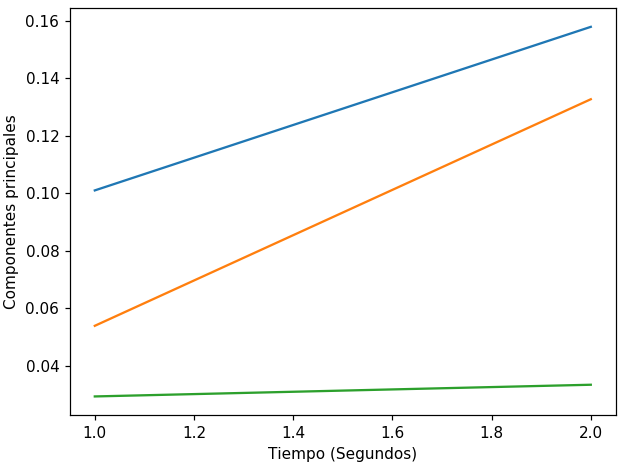
\includegraphics[width=\textwidth]{imagenes/Cap4/pca3-2}
            \caption{Serie de tiempo de 2 pasos.}
            \label{fig:min_max}
        \end{subfigure}       
        \begin{subfigure}[h]{0.45\textwidth} 
            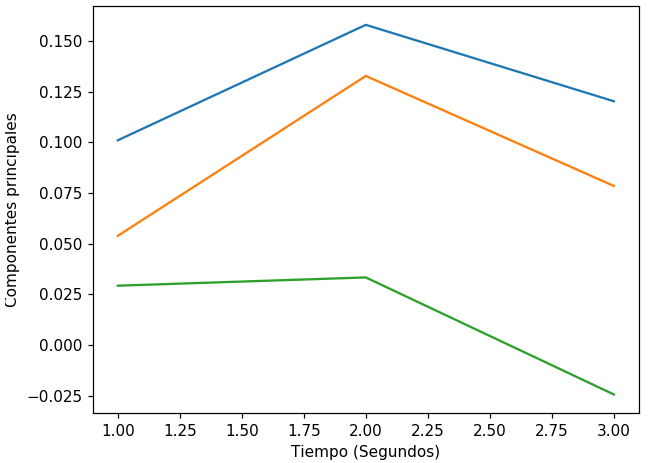
\includegraphics[width=\textwidth]{imagenes/Cap4/pca3-3}
            \caption{Serie de tiempo de 3 pasos.}
            \label{fig:standard}
        \end{subfigure}
        
        \begin{subfigure}[h]{0.45\textwidth} 
            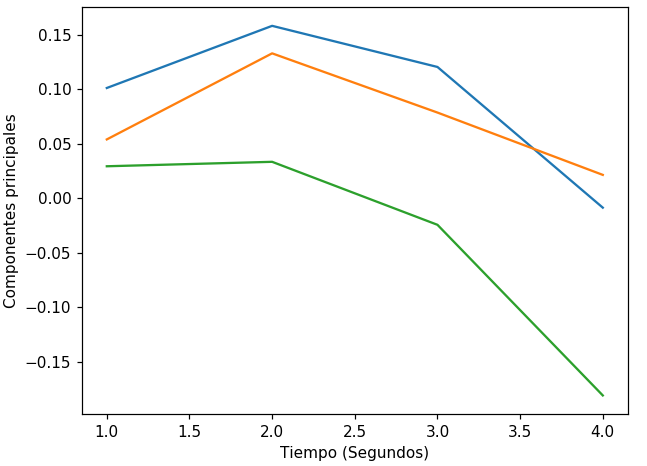
\includegraphics[width=\textwidth]{imagenes/Cap4/pca3-4}
            \caption{Serie de tiempo de 4 pasos.}
            \label{fig:max}
        \end{subfigure}       
        \begin{subfigure}[h]{0.45\textwidth} 
            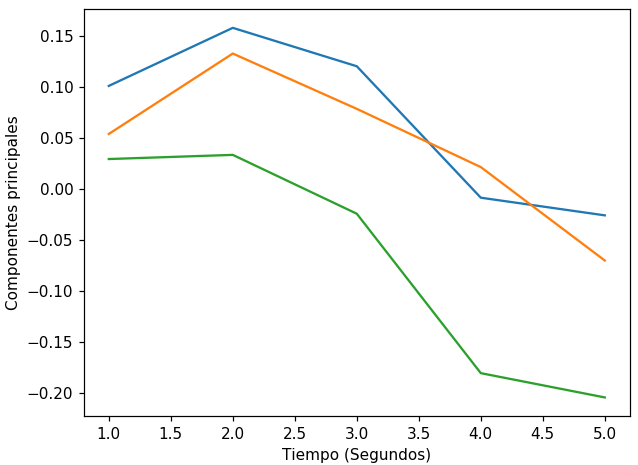
\includegraphics[width=\textwidth]{imagenes/Cap4/pca3-5}
            \caption{Serie de tiempo de 5 pasos.}
            \label{fig:robust}
        \end{subfigure}
        \end{varwidth}}
        \caption{Gr\'{a}fica resultante de diferentes tama\~{n}os de series de tiempo.}
        
		\label{fig:series-de-tiempo}
    \end{figure}
\section{Modelo de detecci\'{o}n de anomal\'{i}as}

La presente investigaci\'{o}n propone un m\'{e}todo de detecci\'{o}n de anomal\'{i}as de conducci\'{o}n siguiendo un enfoque semi-supervisado, el cual consta de dos componentes: un \textbf{modelo del comportamiento normal} y un \textbf{m\'{e}todo para la detecci\'{o}n de valores at\'{i}picos}.

\vspace{5mm} %5mm vertical space

Por lo tanto, se realiz\'{o} la comparaci\'{o}n entre 3 diferentes m\'{e}todos de detecci\'{o}n, y seg\'{u}n el rendimiento de cada uno se elegi\'{o} la mejor opci\'{o}n. En el Cuadro \ref{table:metodos_comparados} se presenta los tres diferentes m\'{e}todos que fueron comparados; donde se puede observar que en todos los casos se usa un autoencoder como modelo del comportamiento normal, de esta manera, las siguientes secci\'{o}nes describir\'{a}n la elecci\'{o}n del autoencoder y la elecci\'{o}n de uno de los tres diferentes m\'{e}todos de detecci\'{o}n de anomal\'{i}as propuestos.

\begin{table}[H]
\centering
\begin{tabular}{|l|p{100mm}|}
\hline
\textbf{M\'{e}todo} & \textbf{Descripci\'{o}n} \\ \hline
AE\_T & M\'{e}todo de detecci\'{o}n basado en autoencoders y umbralizaci\'{o}n (Thresholding). \\ \hline
AE\_IF & M\'{e}todo de detecci\'{o}n basado en autoencoders y aplicaci\'{o}n de Isolation Forest.  \\ \hline
AE\_OC-SVM & M\'{e}todo de detecci\'{o}n basado en autoencoders y aplicaci\'{o}n de One-Class SVM. \\ \hline
\end{tabular}
\caption{Tabla de los m\'{e}todos comparados.}
\label{table:metodos_comparados}
\end{table}

\subsection{Modelo del comportamiento normal}

Esta etapa es una de las partes m\'{a}s importantes de \'{e}ste trabajo, debido a que el rendimiendo del modelo de detecci\'{o}n de anomal\'{i}as depende en gran parte de la precisi\'{o}n de esta etapa.

\subsubsection{Arquitectura del modelo}

Como se mencion\'{o} en la anterior secci\'{o}n en esta etapa se utilizar\'{a} un autoencoder como modelo ajustado al comportamiento normal de conducci\'{o}n. Por lo cual el autoencoder se entren\'{o} con el conjunto de datos normales, de manera que el modelo aprenda a generar s\'{o}lo las clases que se consideran normales y, con suerte, tendr\'{a} problemas para reconstruir anomal\'{i}as, debido a que estas muestras no fueron presentadas durante el entrenamiento.

\vspace{5mm} %5mm vertical space

Para ello se prob\'{o} con diferentes arquitecturas, primero la forma m\'{a}s simple que s\'{o}lo se basa el uso de capas densas (completamente conectadas), luego se hizo pruebas con redes convolucionales y por \'{u}ltimo con redes recurrentes haciendo uso espec\'{i}fico de capas LSTM. Por cada tipo de red se hizo la prueba con 3 diferentes tipos de entrada, es decir, se prob\'{o} una diferente cantidad de pasos (entre 3 y  5) en las series temporales. Por lo tanto se realizaron 9 diferentes experimentos, de los cuales por cada tipo de red sobresali\'{o} una (usando la precisi\'{o}n de las redes como tipo de evaluaci\'{o}n para desarrollar las comparaciones).

\vspace{5mm} %5mm vertical space

En el Cuadro \ref{table:dense33} se presenta la red que obtuvo el mejor resultado de todas las Redes Densas que se probaron, esta red corresponde a la red que fue alimentada con secuencias de 3 pasos. Esta red cuenta con una capa de entrada (Input), una capa de aplanamiento (Flatten) esto debido a que la capa de entrada recibe una entrada bidimensional, un conjunto de capas densas (Dense) que van comprimiendo la informaci\'{o}n de los datos de entrada para posteriormente reconstruirlos, y por \'{u}ltimo la capa de salida es solo una capa para modificar la forma de la salida (Reshape); otro punto importante a resaltar es que las capas internas usan $elu$ como funci\'{o}n de activaci\'{o}n y la \'{u}ltima capa densa utilizan una funci\'{o}n de activaci\'{o}n tangencial ($tanh$), esto se debe a que el conjunto de datos, posterior a la obtenci\'{o}n de componentes principales, se encuentra en el rango $(1, -1)$.

\begin{table}[H]
\centering
\begin{center}
\begin{tabular}{ll|l|r|l|r|}
\cline{3-6}
                                                    &                             & \multicolumn{4}{c|}{\textbf{Arquitectura Densa}}                                                                                                           \\ \cline{3-6} 
                                                    &                             & \multicolumn{4}{c|}{\textbf{NN\_33}}                                                                                                                                   \\ \cline{3-6} 
                                                    &                             & \multicolumn{1}{c|}{\textbf{Tipo}} & \multicolumn{1}{c|}{\textbf{Salida}} & \multicolumn{1}{c|}{\textbf{Activaci\'{o}n}} & \multicolumn{1}{l|}{\textbf{\# Par\'{a}metros}} \\ \hline
\multicolumn{1}{|l|}{\multirow{7}{*}{\textbf{PCA}}} & \multirow{7}{*}{\textbf{3}} & Input                              & (3,3)                                &                                          & 0                                           \\ \cline{3-6} 
\multicolumn{1}{|l|}{}                              &                             & Flatten                            & 9                                    &                                          & 0                                           \\ \cline{3-6} 
\multicolumn{1}{|l|}{}                              &                             & Dense                              & 8                                   & elu                                     & 80                                          \\ \cline{3-6} 
\multicolumn{1}{|l|}{}                              &                             & Dense                              & 5                                   & elu                                     & 45                                          \\ \cline{3-6} 
\multicolumn{1}{|l|}{}                              &                             & Dense                              & 8                                    & elu                                     & 88                                          \\ \cline{3-6} 
\multicolumn{1}{|l|}{}                              &                             & Dense                              & 9                                    & tanh                                     & 81                                          \\ \cline{3-6} 
\multicolumn{1}{|l|}{}                              &                             & Reshape                            & (3,3)                                &                                          & 0                                           \\ \hline
\end{tabular}
\end{center}
\caption{Arquitectura densa para una secuencia de 3 pasos y 3 componentes principales}
\label{table:dense33}
\end{table}

% ejemplos de cuadros de aruqitecturas de redes https://webthesis.biblio.polito.it/10360/1/tesi.pdf

% metricas de evaluacion http://www.diva-portal.org/smash/get/diva2:1225367/FULLTEXT01.pdf  , https://escholarship.org/content/qt1f03f6hb/qt1f03f6hb.pdf  ,   http://www.nada.kth.se/~ann/exjobb/maxim_wolpher.pdf

% Ejemplo cuadros resultados    https://arxiv.org/pdf/1809.00957.pdf 

Por otra parte el Cuadro \ref{table:cnn33} se presenta la red que obtiene la mejor precisi\'{o}n de todas las Redes Convolucionales que fueron probadas, esta red al igual que la anterior corresponde a la red que fue alimentada con secuencias de 3 pasos. Su arquitectura consta de una capa de entrada (Input), una combinaci\'{o}n de capas de convoluci\'{o}n de una dimensi\'{o}n (Conv1D) y agrupaci\'{o}n (MaxPooling1D) hasta comprimir los datos a una dimensi\'{o}n de (2,4), luego un conjunto de capas convolucionales y de muestra ascendente (Upsampling1D) para decodificar la informaci\'{o}n compresa. Cabe recalcar que esta red tambi\'{e}n usa la funci\'{o}n de activaci\'{o}n tangencial en su \'{u}ltima capa por las razones que se explicaron en el p\'{a}rrafo anterior.

\begin{table}[H]
\centering
\begin{center}
\begin{tabular}{ll|l|r|l|r|}
\cline{3-6}
                                                    &                             & \multicolumn{4}{c|}{\textbf{Arquitectura Convolucional}}                                                                                                           \\ \cline{3-6} 
                                                    &                             & \multicolumn{4}{c|}{\textbf{CNN\_33}}                                                                                                                                  \\ \cline{3-6} 
                                                    &                             & \multicolumn{1}{c|}{\textbf{Tipo}} & \multicolumn{1}{c|}{\textbf{Salida}} & \multicolumn{1}{c|}{\textbf{Activaci\'{o}n}} & \multicolumn{1}{l|}{\textbf{\# Par\'{a}metros}} \\ \hline
\multicolumn{1}{|l|}{\multirow{8}{*}{\textbf{PCA}}} & \multirow{8}{*}{\textbf{3}} & Input                              & (3,3)                                &                                          & 0                                           \\ \cline{3-6} 
\multicolumn{1}{|l|}{}                              &                             & Conv1D                             & (3,2)                                & elu                                     & 20                                          \\ \cline{3-6} 
\multicolumn{1}{|l|}{}                              &                             & MaxPooling1D                       & (2,2)                                &                                          & 0                                           \\ \cline{3-6} 
\multicolumn{1}{|l|}{}                              &                             & Conv1D                             & (2,4)                                & elu                                     & 28                                          \\ \cline{3-6} 
\multicolumn{1}{|l|}{}                              &                             & MaxPooling1D                       & (1,4)                                &                                          & 0                                           \\ \cline{3-6} 
\multicolumn{1}{|l|}{}                              &                             & Conv1D                             & (1,6)                                & elu                                     & 54                                          \\ \cline{3-6} 
\multicolumn{1}{|l|}{}                              &                             & UpSampling1D                       & (3,6)                                &                                          & 0                                           \\ \cline{3-6} 
\multicolumn{1}{|l|}{}                              &                             & Conv1D                             & \multicolumn{1}{l|}{(3,3)}           & tanh                                     & 57                                          \\ \hline
\end{tabular}
\end{center}
\caption{Arquitectura convolucional para una secuencia de 3 pasos y 3 componentes principales}
\label{table:cnn33}
\end{table}

% lstm autoencode

En el Cuadro \ref{table:rnn33} se muestra la red que obtuvo la mejor presici\'{o}n de todas las Redes Recurrentes probadas, como en los anteriores casos \'{e}sta red es alimentada con secuencias de 3 pasos. Dicha red cuenta con una capa de entrada (Input), dos capas LSTM una que retorna sus secuencias y una que no, luego viene una capa de redimensionado, posteriormente dos capas LSTM, y finalmente un contenedor  (TimeDistributed) de una capa densa.

\begin{table}[H]
\centering
\begin{center}
\begin{tabular}{ll|l|r|l|r|}
\cline{3-6}
                                                    &                             & \multicolumn{4}{c|}{\textbf{Arquitectura Recurrente}}                                                                                                           \\ \cline{3-6} 
                                                    &                             & \multicolumn{4}{c|}{\textbf{RNN\_33}}                                                                                                                                  \\ \cline{3-6} 
                                                    &                             & \multicolumn{1}{c|}{\textbf{Tipo}} & \multicolumn{1}{c|}{\textbf{Salida}} & \multicolumn{1}{c|}{\textbf{Activaci\'{o}n}} & \multicolumn{1}{l|}{\textbf{\# Par\'{a}metros}} \\ \hline
\multicolumn{1}{|l|}{\multirow{7}{*}{\textbf{PCA}}} & \multirow{7}{*}{\textbf{3}} & Input                              & (3,3)                                &                                          & 0                                           \\ \cline{3-6} 
\multicolumn{1}{|l|}{}                             &                             & LSTM                               & (3,9)                                & elu                                     & 468                                         \\ \cline{3-6} 
\multicolumn{1}{|l|}{}                              &                             & LSTM                               & 6                                    & elu                                     & 384                                         \\ \cline{3-6} 
\multicolumn{1}{|l|}{}                              &                             & Reshape                            & (3,2)                                &                                          & 0                                           \\ \cline{3-6} 
\multicolumn{1}{|l|}{}                              &                             & LSTM                               & (3,3)                                & elu                                     & 72                                          \\ \cline{3-6} 
\multicolumn{1}{|l|}{}                              &                             & LSTM                               & (3,9)                                & elu                                     & 468                                         \\ \cline{3-6} 
\multicolumn{1}{|l|}{}                              &                             & TimeDistributed(Dense)             & (3,3)                                & tanh                                     & 30                                          \\ \hline
\end{tabular}
\end{center}
\caption{Arquitectura recurrente para una secuencia de 3 pasos y 3 componentes principales}
\label{table:rnn33}
\end{table}

Es importante recalcar que las capas de redimensi\'{o}n, agrupaci\'{o}n, muestra ascendente y contenedores s\'{o}lo fueron usadas para controlar la correcta compresi\'{o}n y descompresi\'{o}n de los autoencoders, es por ello que no se detalla a pronfundidad su funcionamiento.

\vspace{5mm} %5mm vertical space

\textbf{Evaluaci\'{o}n de autoencoders}

\vspace{5mm} %5mm vertical space

Anteriormente se present\'{o} los mejores representantes por tipo de red; ahora se proceder\'{a} a la evaluaci\'{o}n y comparaci\'{o}n de estos 3 tipos de autoencoders, con el objetivo de elegir la arquitectura que se ajusta mejor al comportamiento normal de conducci\'{o}n.

\vspace{5mm} %5mm vertical space

En el Cap\'{i}tulo 3 se present\'{o} los diversos tipos de evaluaci\'{o}n que existen, en esta etapa el tipo de evaluaci\'{o}n m\'{a}s apropiado es la \textbf{precisi\'{o}n} del modelo, debido a que se tiene un gran conjunto de datos balanceado (debido a que s\'{o}lo se cuenta con comportamientos normales de conducci\'{o}n que correspoden a una sola clase, la "Normal"). Los resultados de la evaluaci\'{o}n de los tres tipos de redes son mostrados en el Cuadro \ref{table:evaluacion_redes}; dicho cuadro presenta la precisi\'{o}n, p\'{e}rdida logar\'{i}tmica y tiempo de ejecuci\'{o}n de cada autoencoder seg\'{u}n el conjunto de prueba; observando estos resultados se puede apreciar que las dos mejores redes son la red densa \textbf{NN\_33} y la red recurrente \textbf{RNN\_33} con presiciones de 90\% aproximadamente, adem\'{a}s de presentar un valor de p\'{e}rdida relativamente bajo en comparaci\'{o}n a la red \textbf{CNN\_33}.

\begin{table}[H]
\centering
\begin{center}
\begin{tabular}{|l|r|r|r|}
\hline
\textbf{Red} & \multicolumn{1}{l|}{\textbf{Precisi\'{o}n}} & \multicolumn{1}{l|}{\textbf{Loss}} & \multicolumn{1}{l|}{\textbf{Tiempo ejecuci\'{o}n}} \\ \hline
NN\_33              & 0.9000740711953905  & 0.003956934471097257  & 26us/step  \\ \hline
CNN\_33             & 0.8437777761353387  & 0.006740666443275081  & 31us/step  \\ \hline
RNN\_33             & 0.8899259290695191  & 0.003611267575787173  & 101us/step \\ \hline
\end{tabular}
\end{center}
\caption{Evaluaci\'{o}n de las redes NN\_33, CNN\_33 y RNN\_33}
\label{table:evaluacion_redes}
\end{table}

Por otra parte la diferencia m\'{a}s grande entre las dos mejores redes (\textbf{NN\_33} y \textbf{RNN\_33}) es el tiempo de ejecuci\'{o}n ya que de la primera es de tan solo 26 segundos/paso y de la segunda es de 101 segundos/paso, debido a estas similitudes entre ambas redes es necesario verificar visualmente los resultados de reconstrucci\'{o}n de cada tipo de red, de tal manera que se pueda elegir la red m\'{a}s adecuada para este problema. 

\vspace{5mm} %5mm vertical space

En la Figura \ref{fig:res_autoencoders} se muestra los resultados de los autoencoders de siete secuencias tomadas aleatoriamente del conjunto de prueba, en la parte superior de cada figura se encuentra la secuencia de entrada y en la inferior la reconstrucci\'{o}n del modelo, como ya se pod\'{i}a esperar la red \textbf{CNN\_33} presenta los peores resultados, lo cual hace que dicha red sea descartada; en cuanto a las dos redes restantes, la red \textbf{NN\_33} presenta reconstrucciones muy similares a las secuencias de entrada, con algunos peque\~{n}os errores; por otra parte \textbf{RNN\_33} presenta errores un poco m\'{a}s notorios que los obtenidos por  \textbf{NN\_33}. Por lo tanto se lleg\'{o} a la conclusi\'{o}n de que la red \textbf{NN\_33} se ajusta mejor al comportamiento normal de coducci\'{o}n, adem\'{a}s de tener la gran ventaja de tener un tiempo de ejecuci\'{o}n mucho menor que el de \textbf{RNN\_33}, lo cual es realmente importante para los sistemas en tiempo real as\'{i} como tambi\'{e}n de aquellos que cuentan con recursos de ejecucion limitados, como es el caso del presente proyecto.

\begin{figure}
        \centering
        
\fbox{\begin{varwidth}{\textwidth}

        \centering
        \begin{subfigure}[h]{0.99\textwidth} 
            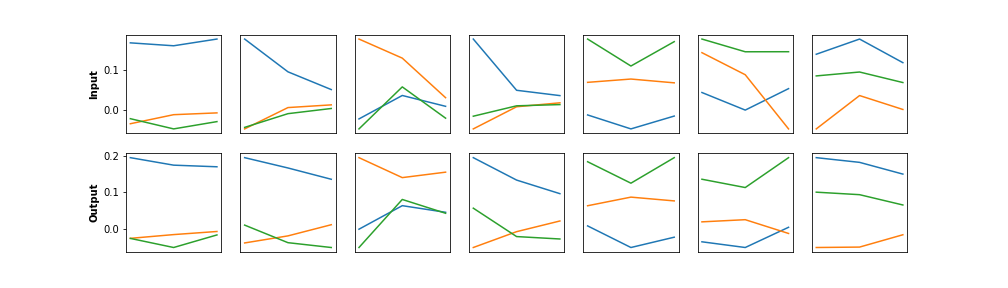
\includegraphics[width=\textwidth]{imagenes/Cap5/resultado_nn}
            \caption{Resultados de la red \textbf{NN\_33}}
            \label{fig:res_nn}
        \end{subfigure}       
        \begin{subfigure}[h]{0.99\textwidth} 
            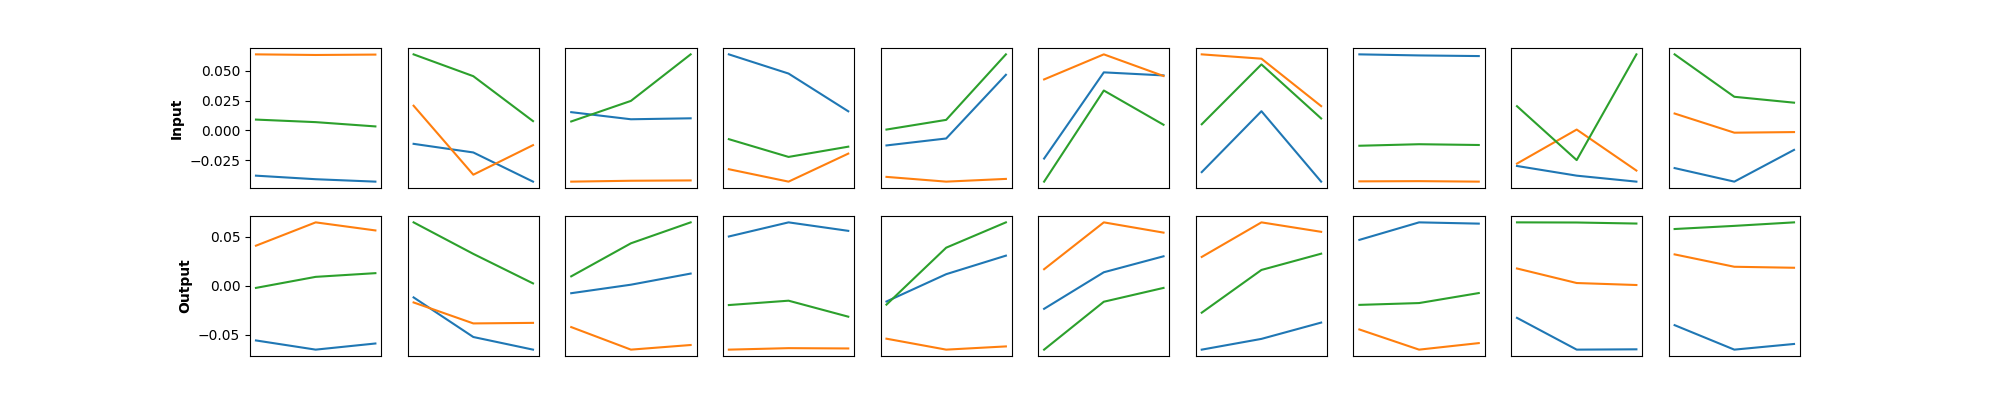
\includegraphics[width=\textwidth]{imagenes/Cap5/resultado_cnn}
            \caption{Resultados de la red \textbf{CNN\_33}}
            \label{fig:res_cnn}
        \end{subfigure}
        
        \begin{subfigure}[h]{0.99\textwidth} 
            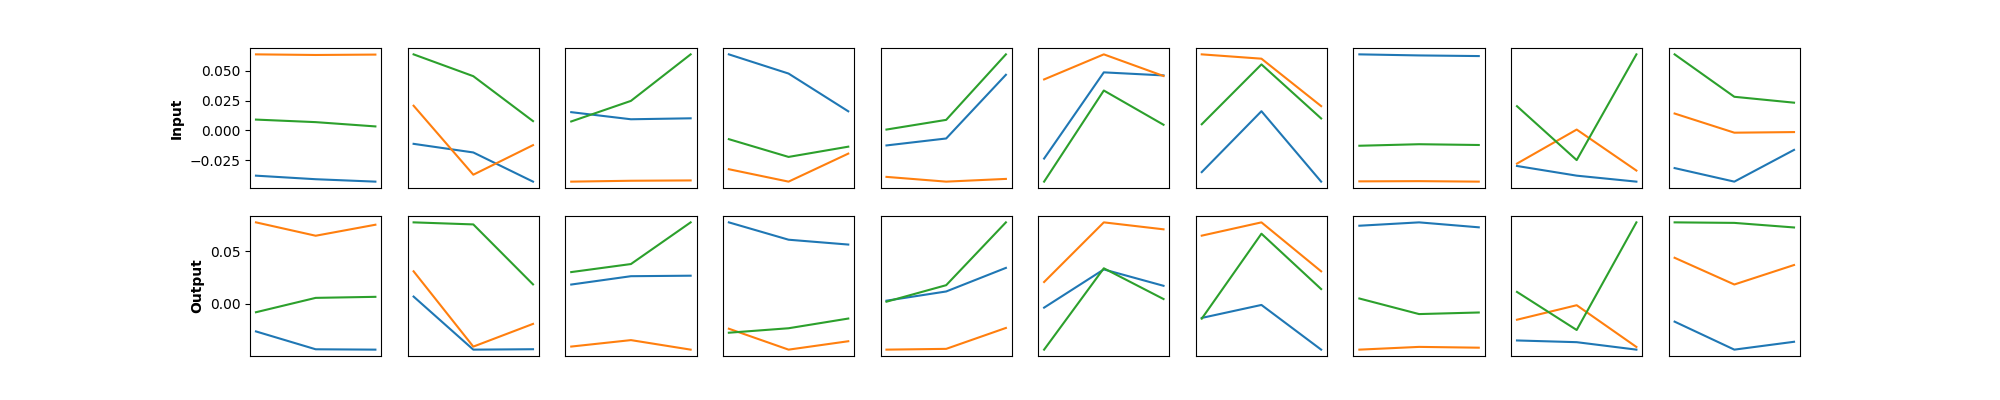
\includegraphics[width=\textwidth]{imagenes/Cap5/resultado_rnn}
            \caption{Resultados de la red \textbf{RNN\_33}}
            \label{fig:res_rnn}
        \end{subfigure}     
        \end{varwidth}}
        \caption{Resultados.}
        
		\label{fig:res_autoencoders}
    \end{figure}


\vspace{5mm} %5mm vertical space

Una vez definido como est\'{a} constituido el modelo del comportamiento normal se puede proceder con la elecci\'{o}n del m\'{e}todo de detecci\'{o}n de valores at\'{i}picos.

\subsection{M\'{e}todo de detecci\'{o}n de anomal\'{i}as}

Al inicio de esta secci\'{o}n se defini\'{o} tres diferentes enfoques para la detecci\'{o}n de anomal\'{i}as: la umbralizaci\'{o}n, la aplicaci\'{o}n de bosques de aislamiento y finalmente la aplicaci\'{o}n de SVM para una clase.

\subsubsection{Umbralizaci\'{o}n}

Esta t\'{e}cnica se basa en la definici\'{o}n de un umbral para determinar si el error de reconstrucci\'{o}n  que obtiene el autoencoder (modelo del comportamiento normal) es lo suficientemente alto como para considerarse un valor at\'{i}pico. Por lo tanto primero se debe definir la ecuaci\'{o}n del error de reconstrucci\'{o}n para el modelo. En el presente trabajo el error de reconstrucci\'{o}n se define seg\'{u}n la ecuaci\'{o}n \ref{eqn:error_rec}, donde $x_{i}$ representa el valor real (entrada del autoencoder) y $\hat{x_{i}}$ representa el valor obtenido por el autoencoder (salida del autoencoder).

\begin{equation}
\textup{Error de reconstrucci\'{o}n} = S_{z} = |x_{i} - \hat{x_{i}}|^{2} 
\label{eqn:error_rec}
\end{equation}

En la Figura \ref{fig:codos} se muestra la curva de los errores de reconstrucci\'{o}n obtenidos con el modelo del compotamiento normal para el conjunto de muestras normales.

\begin{figure}[H]
        \centering
            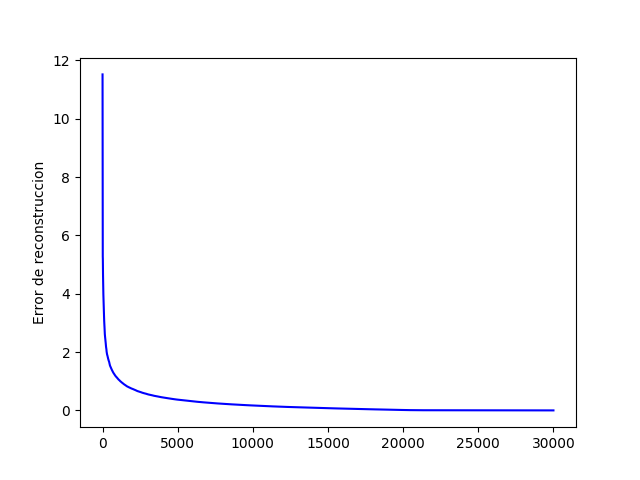
\includegraphics[width=0.75\textwidth, frame]{imagenes/Cap5/codos}
        \caption{Curva de los valores de reconstrucci\'{o}n obtenidos con el modelo del comportamiento normal.}
		\label{fig:codos}
    \end{figure}

Una vez definido la ecuaci\'{o}n de reconstrucci\'{o}n, se debe definir un umbral capaz de poder detectar la mayor cantidad de anomal\'{i}as posibles. Esta tarea puede tornarse simple en un entorno de aprendizaje supervisado, sin embargo automatizar esta tarea en un contexto de aprendizaje no supervisado es un desafio que puede ser dificil de sobrellevar. En el presente trabajo se uso una t\'{e}cnica basada en encontrar un \textit{Punto de codo} de una curva, que en este caso la curva est\'{a} construida en base a los errores de reconstrucci\'{o}n del autoencoder.

\vspace{5mm} %5mm vertical space

% https://github.com/arvkevi/kneed
Existen diferentes formas de hallar el punto de codo, sin embargo en este trabajo se utiliz\'{o} una herramienta de Python, que automatiza esta tarea, llamada Kneedle. Esta herramienta devuelve el punto de inflexi\'{o}n de la funci\'{o}n de la curva obtenida por el conjunto de valores proporcionado \textit{x} y \textit{y}, cabe recalcar que el punto de codo es el punto de m\'{a}xima curvatura, por otra parte esta herramienta cuenta con un par\'{a}metro de sensibilidad (S), este par\'{a}metro permite ajustar qu\'{e} tan agresivo se desea ser al detectar codos, los valores m\'{a}s peque\~{n}os para S detectan los codos m\'{a}s r\'{a}pido, mientras que los m\'{a}s grandes son m\'{a}s conservadores, es decir, S es una medida de cu\'{a}ntos puntos ''planos'' se espera ver en la curva de datos sin modificar antes de declarar un codo.

\vspace{5mm} %5mm vertical space

De esta manera en el presente proyecto se realiz\'{o} experimentos con diferentes valores de sensibilidad para encontrar el codo m\'{a}s adecuado para nuestro conjunto de datos. En la Figura \ref{fig:zoom_codos}, se muestra los diferentes codos hallados para los valores de sensibilidad proporcionados (valores entre 0 y 2).

\begin{figure}[H]
        \centering
            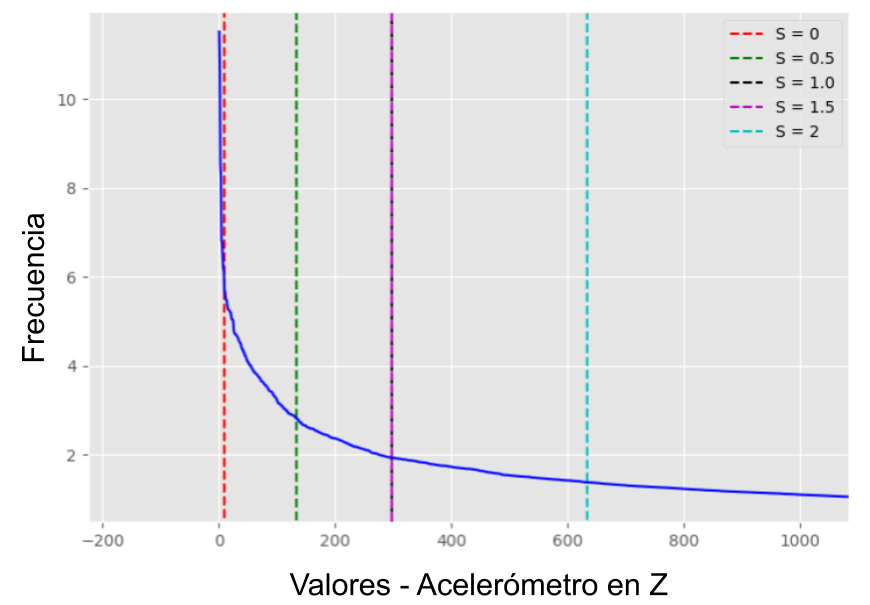
\includegraphics[width=0.75\textwidth, frame]{imagenes/Cap5/zoom_codos}
        \caption{Resultados de la obtenci\'{o}n de codos con diferentes valores de Sensibilidad, para los valores de reconstrucci\'{o}n obtenidos con el modelo del comportamiento normal.}
		\label{fig:zoom_codos}
\end{figure}

Una vez obtenidos los codos se realiz\'{o} la evaluaci\'{o}n de cada uno de ellos, en el Cuadro \ref{table:evaluacion_codos} se presentan el umbral, los valores de la matriz de confusi\'{o}n, la sensibilidad y especifidad para cada codo. Los valores de la matriz de confusi\'{o}n son el resultado de aplicar el umbral de cada codo a los errores de reconstrucci\'{o}n obtenidos del conjunto de datos total (conjunto de datos normal y anormal equivalente a 44204 datos).

\begin{table}[H]
\centering
\begin{center}
\begin{tabular}{|l|r|r|r|r|r|r|r|}
\hline
\textbf{S} & \multicolumn{1}{l|}{\textbf{Umbral}} & \multicolumn{1}{l|}{\textbf{VP}} & \multicolumn{1}{l|}{\textbf{VN}}& \multicolumn{1}{l|}{\textbf{FN}}& \multicolumn{1}{l|}{\textbf{FP}} & \multicolumn{1}{l|}{\textbf{Sensibilidad}} & \multicolumn{1}{l|}{\textbf{Especificidad}} \\ \hline
0.0 & 5.665 & \cellcolor[HTML]{AADD99} 92 & \cellcolor[HTML]{AADD99} 43993 & \cellcolor[HTML]{FFCE93} 72 & \cellcolor[HTML]{FFCE93} 47 & 0.5610 & 0.9989 \\ \hline
0.5  & 2.806 & \cellcolor[HTML]{AADD99} 111 & \cellcolor[HTML]{AADD99} 43814 & \cellcolor[HTML]{FFCE93} 53 & \cellcolor[HTML]{FFCE93} 226 & 0.6768 & 0.9949 \\ \hline
1.0 &  1.920 & \cellcolor[HTML]{AADD99} 120 & \cellcolor[HTML]{AADD99} 43562 & \cellcolor[HTML]{FFCE93} 44 & \cellcolor[HTML]{FFCE93} 478 & 0.7317 & 0.9891 \\ \hline
2.0 & 1.369	 & \cellcolor[HTML]{AADD99} 128 & \cellcolor[HTML]{AADD99} 43100  & \cellcolor[HTML]{FFCE93} 36 & \cellcolor[HTML]{FFCE93} 940 & 0.7805 & 0.9787 \\ \hline
\end{tabular}
\end{center}
\caption{Evaluaci\'{o}n de la detecci\'{o}n de anomal\'{i}as para cada codo obtenido con los diferentes valores de sensibilidad.}
\label{table:evaluacion_codos}
\end{table}

Seg\'{u}n los resultados que se muestran en el Cuadro \ref{table:evaluacion_codos} se puede decir que mientras m\'{a}s peque\~{n}o es el umbral la sensibilidad (proporci\'{o}n de anomal\'{i}as detectadas correctamente como anomal\'{i}as) incrementa, sin embargo, a su vez reduce la especifidad (proporci\'{o}n de valores normales correctamente detectados como valores normales). Por lo tanto se debe hallar un punto intermedio, donde se pueda detectar la mayor cantidad de anomal\'{i}as posibles y reducir en lo posible la cantidad de falsos positivos (datos normales que son detectados como anomal\'{i}as). De esta forma el umbral m\'{a}s adecuado para el objetivo planteado fue 2.806, ya que con este umbral se detecta 111 anomal\'{i}as de 164 y los falsos positivos son aproximadamente el doble de los valores at\'{i}picos detectados. 

\vspace{5mm} %5mm vertical space

De ello se deduce que, para detectar autom\'{a}ticamente el umbral el uso de 0.5 como par\'{a}metro S es el m\'{a}s adecuado, sin embargo si se desea incrementar el porcentaje de detecci\'{o}n de anomal\'{i}as a costa de incrementar el n\'{u}mero de falsos positivos se puede usar un valor mayor a 0.5 para S y en caso de querer la menor cantidad de falsos positivos posibles se debe usar un valor menor a 0.5.

\subsubsection{Isolation Forest}

Antes de presentar como se llevar\'{a} a cabo los experimentos con este algoritmo, es necesario ilustrar m\'{a}s detalladamente el funcionamiento del mismo. Por lo tanto la Figura \ref{fig:isolartion-forest} representa c\'{o}mo se espera que un punto de datos anómalo se aísle rápidamente con el uso de este algoritmo, mientras que un punto de datos normal necesita más particiones para poder ser aislado.

\begin{figure}[h!]
  \begin{center}	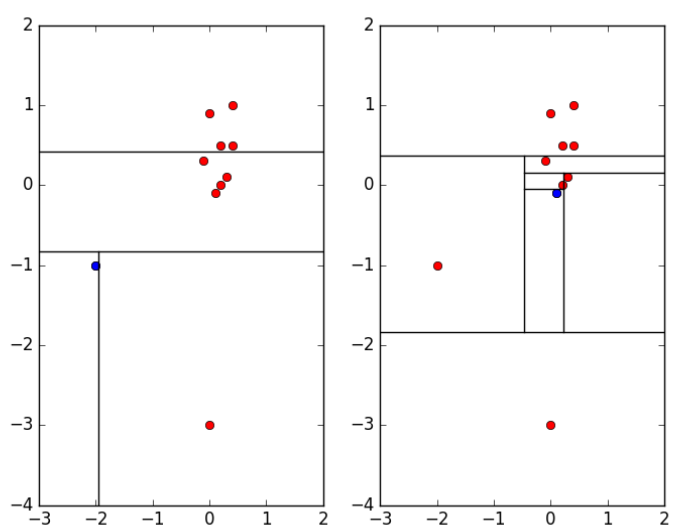
\includegraphics[width=0.75\textwidth, frame]{imagenes/Cap5/isolation-forest}
  \caption{La figura de la izquierda muestra el aislamiento de una anomalía, que requiere solo tres particiones. A la derecha, el aislamiento de un punto normal requiere seis particiones \protect\cite{Reference60}.} 
  \label{fig:isolartion-forest}
  \end{center}
\end{figure}

Una vez detallado resumidamente el funcionamiento de los bosques de aislamiento se puede proseguir con los diferentes enfoques de los experimentos que se realizar\'{a} con Isolation Forest.

\vspace{5mm} %5mm vertical space

Existen dos enfoques que pueden realizarse con esta t\'{e}cnica; el primero entrena el modelo con los valores compresos del codificador del autoencoder y el segundo se entrena con los errores de reconstrucci\'{o}n del autoencoder. A continuaci\'{o}n se presenta una gr\'{a}fica (Ver Figura \ref{fig:autoencoder}) del autoencoder (modelo del comportamiento normal) con el fin de tener un mejor entendimiento de c\'{o}mo se realizar\'{a}n los experimentos tanto para los bosques de aislamiento como para los SVM de una clase.

\begin{figure}[H]
        \centering
            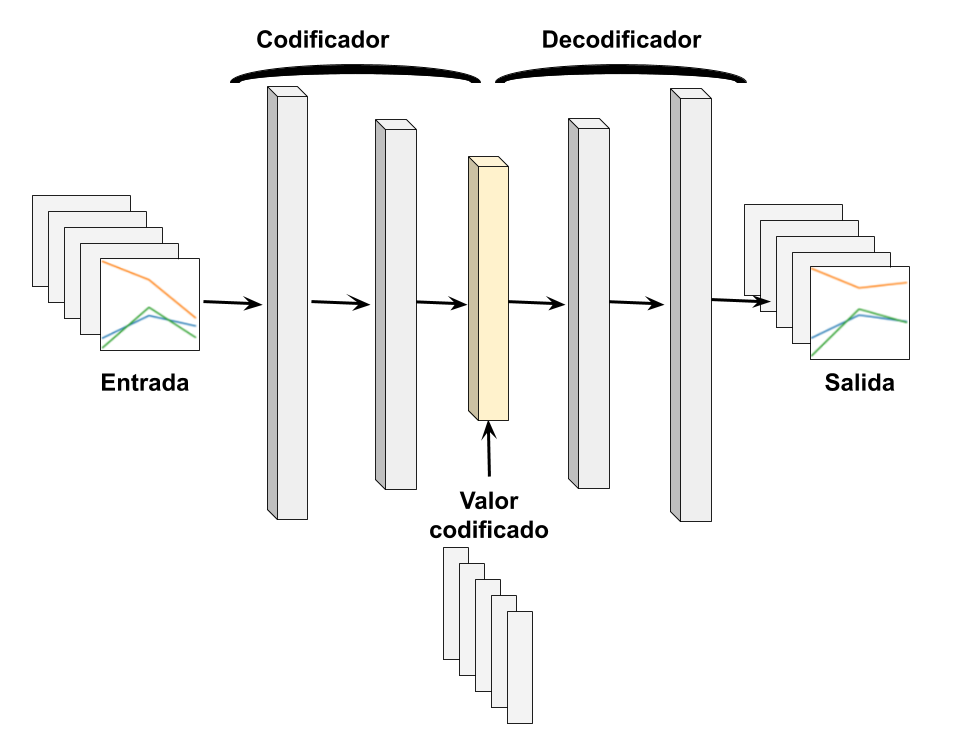
\includegraphics[width=0.75\textwidth, frame]{imagenes/Cap5/autoencoder}
        \caption{Representaci\'{o}n gr\'{a}fica del modelo de comportamiento normal o autoencoder.}
		\label{fig:autoencoder}
\end{figure}

\begin{itemize}
\item \textbf{\textit{Isolation forest para valores codificados: }}Esta t\'{e}cnica entrena un modelo de bosque de aislamiento con los valores codificados (mediante el codificador del autoencoder, ver Figura \ref{fig:autoencoder}) del conjunto de entrenamiento normal. Para los experimentos se utiliz\'{o} la clase IsolationForest de \textsc{scikit-learn}, esta clase tiene un par\'{a}metro llamado \textsc{contaminaci\'{o}n} el cual sirve para definir que cantidad del conjunto de datos esta contamiado, es decir, define que cantidad de los datos de entrenamiento pueden ser valores at\'{i}picos; en la presente investigaci\'{o}n se realiz\'{o} varias pruebas con diferentes valores para el par\'{a}metro contaminaci\'{o}n. En el Cuadro \ref{table:evaluacion_IF_encoded} se presenta los resultados, donde se evidencia que ninguno de los resultados es alentador, ya que la cantidad de anomal\'{i}as detectadas es muy baja para los tres casos con los que se experimento.

\begin{table}[H]
\centering
\begin{center}
\begin{tabular}{|l|r|r|r|r|r|r|r|}
\hline
\textbf{Contaminaci\'{o}n (C)} & \multicolumn{1}{l|}{\textbf{VP}} & \multicolumn{1}{l|}{\textbf{VN}}& \multicolumn{1}{l|}{\textbf{FN}}& \multicolumn{1}{l|}{\textbf{FP}} & \multicolumn{1}{l|}{\textbf{Sensibilidad}} & \multicolumn{1}{l|}{\textbf{Especificidad}} \\ \hline
0.0025 & \cellcolor[HTML]{AADD99} 3 & \cellcolor[HTML]{AADD99} 43944 & \cellcolor[HTML]{FFCE93} 161 & \cellcolor[HTML]{FFCE93} 96 & 0.0183 & 0.9978 \\ \hline
0.0050 & \cellcolor[HTML]{AADD99} 17 & \cellcolor[HTML]{AADD99} 43817 & \cellcolor[HTML]{FFCE93} 147 & \cellcolor[HTML]{FFCE93} 223 & 0.1037 & 0.9949 \\ \hline
0.0075 & \cellcolor[HTML]{AADD99} 17 & \cellcolor[HTML]{AADD99} 43738 & \cellcolor[HTML]{FFCE93} 147 & \cellcolor[HTML]{FFCE93} 302 & 0.1037 & 0.9931 \\ \hline
\end{tabular}
\end{center}
\caption{Evaluaci\'{o}n de la detecci\'{o}n de anomal\'{i}as usando Isolation forest para valores compresos.}
\label{table:evaluacion_IF_encoded}
\end{table}

\item \textbf{\textit{Isolation forest para errores de reconstrucci\'{o}n: }}Para esta t\'{e}cnica se realiz\'{o} el entrenamiento del bosque de aislamiento con la diferencia de los valores de entrada con los valores obtenidos por el autoencoder (Ver Figura \ref{fig:error}), cabe aclarar que la diferencia mencionada anteriormente tambi\'{e}n ser\'{a} llamada \textit{Error de reconstrucci\'{o}n} tanto en esta como en la siguiente subsecci\'{o}n. Los resultados de esta t\'{e}cnica para diferentes valores de contaminaci\'{o}n se presentan en el Cuadro \ref{table:evaluacion_IF_errores_reconstruccion}, donde estos resultados se pueden consider como \'{o}ptimos, debido a que oscilan entre 62 y 67\% de detecci\'{o}nes correctas de anomal\'{i}as, adem\'{a}s de presentar una especificidad realmente alta, del 99\% aproximadamente, lo cual quiere decir que estos modelos presentan una baja tasa de falsos positivos. 

\begin{figure}[H]
        \centering
            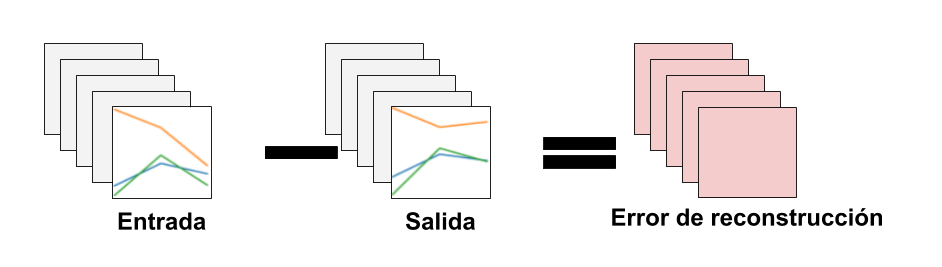
\includegraphics[width=0.75\textwidth, frame]{imagenes/Cap5/error}
        \caption{Representaci\'{o}n gr\'{a}fica del error de reconstrucci\'{o}n usado para el entrenamiento de los bosques de aislamiento y los SVM de una clase.}
		\label{fig:error}
\end{figure}

\begin{table}[H]
\centering
\begin{center}
\begin{tabular}{|l|r|r|r|r|r|r|r|}
\hline
\textbf{Contaminaci\'{o}n (C)} & \multicolumn{1}{l|}{\textbf{VP}} & \multicolumn{1}{l|}{\textbf{VN}}& \multicolumn{1}{l|}{\textbf{FN}}& \multicolumn{1}{l|}{\textbf{FP}} & \multicolumn{1}{l|}{\textbf{Sensibilidad}} & \multicolumn{1}{l|}{\textbf{Especificidad}} \\ \hline
0.0025 & \cellcolor[HTML]{AADD99} 103 & \cellcolor[HTML]{AADD99} 43898 & \cellcolor[HTML]{FFCE93} 61 & \cellcolor[HTML]{FFCE93} 142 & 0.6280 & 0.9968 \\ \hline
0.0050 & \cellcolor[HTML]{AADD99} 108 & \cellcolor[HTML]{AADD99} 43792 & \cellcolor[HTML]{FFCE93} 56 & \cellcolor[HTML]{FFCE93} 248 & 0.6585 & 0.9944 \\ \hline
0.0075 & \cellcolor[HTML]{AADD99} 111 & \cellcolor[HTML]{AADD99} 43688 & \cellcolor[HTML]{FFCE93} 53 & \cellcolor[HTML]{FFCE93} 352 & 0.6768 & 0.9920 \\ \hline
\end{tabular}
\end{center}
\caption{Evaluaci\'{o}n de la detecci\'{o}n de anomal\'{i}as usando Isolation forest para errores de reconstrucci\'{o}n.}
\label{table:evaluacion_IF_errores_reconstruccion}
\end{table}
\end{itemize}

\subsubsection{One-Class SVM}

De la misma forma que en los bosques de aislamiento, se realiz\'{o} dos diferentes tipos de experimentos con One-Class SVM, a continuaci\'{o}n se detalla cada uno de ellos.

\begin{itemize}
\item \textbf{\textit{One-Class SVM para valores codificados: }}Se debe entrenar un modelo SVM de una clase para los valores compresos obtenidos por el autoencoder; los experimentos fueron realizados usando la clase OneClassSVM de \textsc{scikit-learn}, donde se tiene diferentes par\'{a}metros que pueden ser personalizados, para la presente investigaci\'{o}n se prob\'{o} diferentes kernels, obteniendo as\'{i} los resultados que se muestran en el Cuadro \ref{table:evaluacion_SVM_encoded}, donde claramente ninguno de los resultados obtenidos podr\'{i}a ser tomado en cuenta para ser el m\'{e}todo de detecci\'{o}n de anomal\'{i}as de conducci\'{o}n ya que la sensibilidad en ninguno de los casos es superior a 50\%.

\begin{table}[H]
\centering
\begin{center}
\begin{tabular}{|l|r|r|r|r|r|r|r|}
\hline
\textbf{Kernel} & \multicolumn{1}{l|}{\textbf{VP}} & \multicolumn{1}{l|}{\textbf{VN}}& \multicolumn{1}{l|}{\textbf{FN}}& \multicolumn{1}{l|}{\textbf{FP}} & \multicolumn{1}{l|}{\textbf{Sensibilidad}} & \multicolumn{1}{l|}{\textbf{Especificidad}} \\ \hline
rbf & \cellcolor[HTML]{AADD99} 49 & \cellcolor[HTML]{AADD99} 41746 & \cellcolor[HTML]{FFCE93} 115 & \cellcolor[HTML]{FFCE93} 2294 & 0.2988 & 0.9479 \\ \hline
poly & \cellcolor[HTML]{AADD99} 56 & \cellcolor[HTML]{AADD99} 22532 & \cellcolor[HTML]{FFCE93} 108 & \cellcolor[HTML]{FFCE93} 21508 & 0.3415 & 0.5116 \\ \hline
sigmoid & \cellcolor[HTML]{AADD99} 13 & \cellcolor[HTML]{AADD99} 42378 & \cellcolor[HTML]{FFCE93} 151 & \cellcolor[HTML]{FFCE93} 1662 & 0.0793 & 0.9623 \\ \hline
\end{tabular}
\end{center}
\caption{Evaluaci\'{o}n de la detecci\'{o}n de anomal\'{i}as usando One-Class SVM para valores compresos.}
\label{table:evaluacion_SVM_encoded}
\end{table}

\item \textbf{\textit{One-Class SVM para los errores de reconstrucci\'{o}n: }}Al igual que uno de los experimentos que se realiz\'{o} con Isolation Forest, en esta t\'{e}cnica se usa los errores de reconstrucci\'{o}n (Ver Figura \ref{fig:error}) para realizar el entrenamiento del modelo SVM de una clase. Como en los experimentos realizados en la anterior t\'{e}cnica se realiz\'{o} diferentes pruebas con distintos tipos de kernel, a continuaci\'{o}n en el Cuadro \ref{table:evaluacion_SVM_error} se presenta los resultados obtenidos en los experimentos.

\begin{table}[H]
\centering
\begin{center}
\begin{tabular}{|l|r|r|r|r|r|r|r|}
\hline
\textbf{Kernel} & \multicolumn{1}{l|}{\textbf{VP}} & \multicolumn{1}{l|}{\textbf{VN}}& \multicolumn{1}{l|}{\textbf{FN}}& \multicolumn{1}{l|}{\textbf{FP}} & \multicolumn{1}{l|}{\textbf{Sensibilidad}} & \multicolumn{1}{l|}{\textbf{Especificidad}} \\ \hline
rbf & \cellcolor[HTML]{AADD99} 134 & \cellcolor[HTML]{AADD99} 41887 & \cellcolor[HTML]{FFCE93} 30 & \cellcolor[HTML]{FFCE93} 2153 & 0.8170 & 0.9511 \\ \hline
poly & \cellcolor[HTML]{AADD99} 97 & \cellcolor[HTML]{AADD99} 1559 & \cellcolor[HTML]{FFCE93} 67 & \cellcolor[HTML]{FFCE93} 42481 & 0.5915 & 0.0354 \\ \hline
sigmoid & \cellcolor[HTML]{AADD99} 123 & \cellcolor[HTML]{AADD99} 1683 & \cellcolor[HTML]{FFCE93} 41 & \cellcolor[HTML]{FFCE93} 42357 & 0.7500 & 0.0382 \\ \hline
\end{tabular}
\end{center}
\caption{Evaluaci\'{o}n de la detecci\'{o}n de anomal\'{i}as usando One-Class SVM para el error de reconstrucci\'{o}n del autoencoder.}

\label{table:evaluacion_SVM_error}
\end{table}


Observando los resultados del Cuadro se puede notar que se aument\'{o} notablemente la sensibilidad, o cantidad de anomal\'{i}as detectadas correctamente, sin embargo, redujo dr\'{a}sticamente la especificidad ya que en algunos casos tan solo llega a un 3.5\%, lo cual es muy alejado al objetivo que se persigue en el presente trabajo.

\end{itemize}

\subsubsection{Evaluaci\'{o}n del m\'{e}todo de detecci\'{o}n de anomal\'{i}as}

Una vez realizado los diferentes tipos de experimentos, se evalu\'{o} el mejor exponente de cada tipo, con el fin de elegir el m\'{a}s adecuado para la investigaci\'{o}n. A continuaci\'{o}n se presenta un Cuadro \ref{table:evaluacion_metodo_anomalias} con los resultados de los mejores representantes por cada tipo de t\'{e}cnica.

\begin{table}[H]
\centering
\begin{center}
\begin{tabular}{|p{40mm}|r|r|r|r|r|r|r|}
\hline
\textbf{Nombre m\'{e}todo} & \multicolumn{1}{l|}{\textbf{VP}} & \multicolumn{1}{l|}{\textbf{VN}}& \multicolumn{1}{l|}{\textbf{FN}}& \multicolumn{1}{l|}{\textbf{FP}} & \multicolumn{1}{l|}{\textbf{Sensibilidad}} & \multicolumn{1}{l|}{\textbf{Especificidad}} \\ \hline
Umbralizaci\'{o}n con S=0.5 & \cellcolor[HTML]{AADD99} 111 & \cellcolor[HTML]{AADD99} 43814 & \cellcolor[HTML]{FFCE93} 53 & \cellcolor[HTML]{FFCE93} 226 & 0.6768 & 0.9949 \\ \hline
Isolation Forest para errores de reconstrucci\'{o}n con C=0.0075 & \cellcolor[HTML]{AADD99} 111 & \cellcolor[HTML]{AADD99} 43688 & \cellcolor[HTML]{FFCE93} 53 & \cellcolor[HTML]{FFCE93} 352 & 0.6768 & 0.9920 \\ \hline
One-Class SVM para errores de reconstrucci\'{o}n con kernel RBF& \cellcolor[HTML]{AADD99} 134 & \cellcolor[HTML]{AADD99} 41887 & \cellcolor[HTML]{FFCE93} 30 & \cellcolor[HTML]{FFCE93} 2153 & 0.8170 & 0.9511 \\ \hline
\end{tabular}
\end{center}
\caption{Comparaci\'{o}n de los mejores m\'{e}todos de detecci\'{o}n de anomal\'{i}as.}

\label{table:evaluacion_metodo_anomalias}
\end{table}

Evidentemente el mejor resultado de detecci\'{o}n de anomal\'{i}as es el que se obtuvo por el modelo SVM para una clase con una sensibilidad del 81.7\%, sin embargo, este m\'{e}todo presenta la desventaja de tener una alta cantidad de falsos positivos, es decir, por cada anomal\'{i}a detectada se tendr\'{a} aproximadamente 13 alertas por falsos positivos, lo cual es una valor muy alto; y es la principal raz\'{o}n por la que se descarta este m\'{e}todo.

\vspace{5mm} %5mm vertical space

Debido a esto s\'{o}lo quedan dos m\'{e}odos a comparar, donde ambos resultados son muy similares; ya que estos cuentan con una sensibilidad de 67.68\%, por otra parte la especificidad tiene una peque\~{n}a variaci\'{o}n entre ambas t\'{e}cnicas dando un resultado levemente mejor para la t\'{e}cnica de umbralizaci\'{o}n con 99.49\% frente a un 99.20\%.

\vspace{5mm} %5mm vertical space

En este punto se puede elegir cualquiera de estos dos m\'{e}todos debido a las similitudes que ambos presentan. Por razones de simplificidad en este estudio se elegi\'{o} el m\'{e}todo de bosque de aislamiento ya que este m\'{e}todo hace m\'{a}s sencilla la detecci\'{o}n de anomal\'{i}as debido a que uno puede especificar la cantidad de contaminaci\'{o}n que se espera del conjunto de datos, esto es mucho m\'{a}s ventajoso que la busqueda de codos con el m\'{e}todo de umbralizaci\'{o}n ya que presenta la desventaja de que es realmente complejo definir el umbral cuando se trata esta t\'{e}cnica en un enfoque no supervisado, como es el caso de esta etapa, adem\'{a}s que la definici\'{o}n del umbral depende mucho de cu\'{a}n limpio o contaminado se encuentra el conjunto de datos, haciendo m\'{a}s complejo el correcto tratamiento al aplicar este m\'{e}todo.

\vspace{5mm} %5mm vertical space

Una vez elegido los mejores m\'{e}todos para conformar el mecanismo de detecci\'{o}n de valores at\'{i}picos, se procede a formalizar este mecanismo por medio de una gr\'{a}fica (Ver Figura \ref{fig:mecanismo}), la cual proporciona una representaci\'{o}n visual del flujo del detector de anomal\'{i}as propuesto; ya que es importante conocer como se compone y como funciona, especialmente antes de realizar su respectiva evalucia\'{o}n. 

\begin{figure}[H]
        \centering
            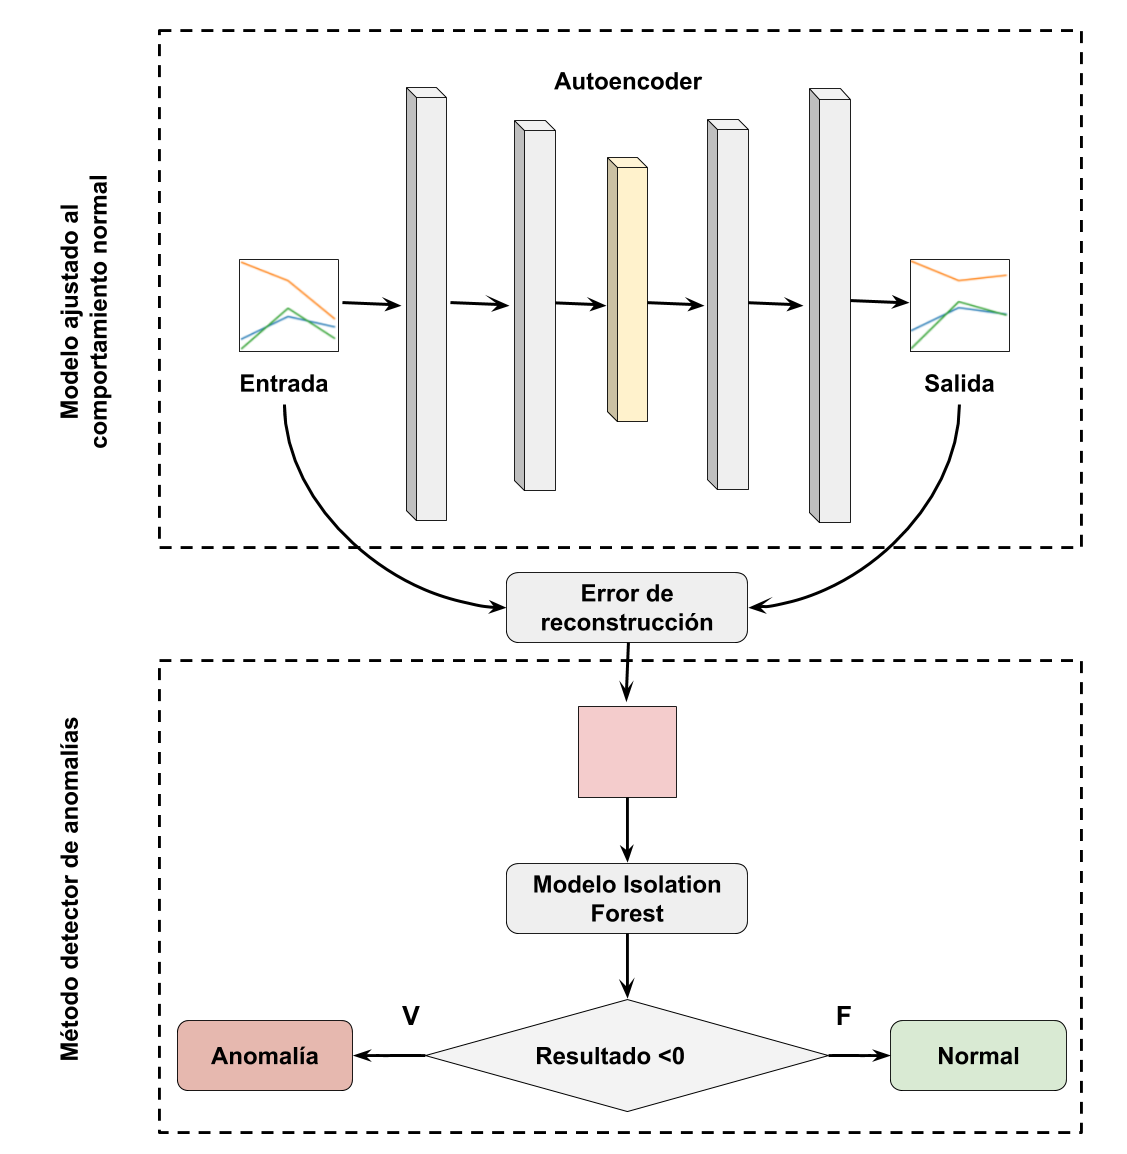
\includegraphics[width=0.92\textwidth, frame]{imagenes/Cap5/mecanismo}
        \caption{Mecanismo de detecci\'{o}n de anomal\'{i}as.}
		\label{fig:mecanismo}
\end{figure}

Observando la Figura \ref{fig:mecanismo}, se puede notar claramente los componentes que conforman el mecanismo de detecci\'{o}n de anomal\'{i}as: el \textbf{modelo del comportamiento normal} y el \textbf{m\'{e}todo detector de anomal\'{i}as}. Este mecanismo funciona de una forma muy sencilla, en primer lugar se proporciona al autoencoder una secuencia de entrada con 3 pasos para 3 componentes principales (cabe aclarar que los datos de entrada han sido previamente pre-procesados), este autoencoder devuelve como salida la reconstrucci\'{o}n de la entrada, con la cual se obtiene el error de reconstrucci\'{o}n (diferencia entre la entrada real y el valor reconstruido), dicho valor es a su vez la entrada del modelo de bosque de aislamiento, el cual puede retornar dos tipos de valores (-1, 1); cuando este modelo retorna el valor 1 quiere decir que la entrada proporcionada corresponde a un valor considerado como normal y en caso de retornar -1 significa que dicha entrada es una anomal\'{i}a, terminando as\'{i} el flujo del mecanismo de detecci\'{o}n propuesto en el presente trabajo.

\section{Resumen}

En este cap\'{i}tulo se ha detallado como est\'{a} conformado el conjunto de valores at\'{i}picos, que herramientas fueron utilizadas para el desarrollo de los experimentos. Por otra parte tambi\'{e}n se describi\'{o} detalladamente todos los tipos de experimentos realizados durante la investigaci\'{o}n y finalmente la elecci\'{o}n de los m\'{e}todos m\'{a}s adecuados para formar parte del mecanismo de detecci\'{o}n de anomal\'{i}as. En el siguiente cap\'{i}tulo se abordar\'{a} un an\'{a}lisis detallado de los resultados obtenidos por el mecanismo de detecci\'{o}n.
 